\section{Introduction and Preliminaries}
%
%
%
%
The QUT HPC facilities provide access to,
\begin{itemize}
\item 212 compute nodes
\item 3780 Intel Xeon Cores
\item Approx. 200G B RAM per Compute Nodes
\item 34 TB of main storage
\item 1800 TB additional storage in file store
\item 24 Tesla GPUs
\item Visualisations services and more
\end{itemize}
%
%
%
\subsection{Getting HPC Access}
Before accessing HPC, you will first need to apply for access. This can be done via HiQ by following the instructions on this link \href{https://qutvirtual4.qut.edu.au/group/research-students/doing-your-research/specialty-research-facilities/apply-for-a-hpc-account}{here}. Access will usually be granted in a couple of days at the most.
%
%
\par
%
%
Once access has been granted, you will need a program to access HPC. If you are using a Linux or Mac, you won't need to install anything, though if you are using Windows, it is recommended to use the program PuTTY \cite{putty}. Instructions on logging in to HPC for each OS are given here.
%
%
\subsubsection{Mac and Linux}
To log into HPC, we will be using the Secure SHell (SSH) protocol, which we can access through the command line on Mac and Linux devices. To login, first open a command line prompt (terminal) in your computer. To login, you will simply need to type in,
\begin{lstlisting}[language=bash, frame=single]
  ssh <your_qut_id>@lyra.qut.edu.au
\end{lstlisting}
where you will replace \texttt{<your\_qut\_id>} with your QUT username, ie.
\begin{lstlisting}[language=bash, frame=single]
  #if you applied for HPC access with staff acount
  ssh jane.doe@lyra.qut.edu.au
  #if you applied for HPC access with student acount
  ssh n12345678@lyra.qut.edu.au
\end{lstlisting}
%
%
%
%
\subsubsection{Windows}
To login on windows, first install PuTTY by following the instructions \href{https://www.putty.org/}{here}. Once downloaded, simply open the putty window and enter \texttt{lyra.qut.edu.au} into the bar as shown in Figure \ref{fig:putty}. You will then have to enter your QUT username and password.
\begin{figure}[!h]
  \centering
  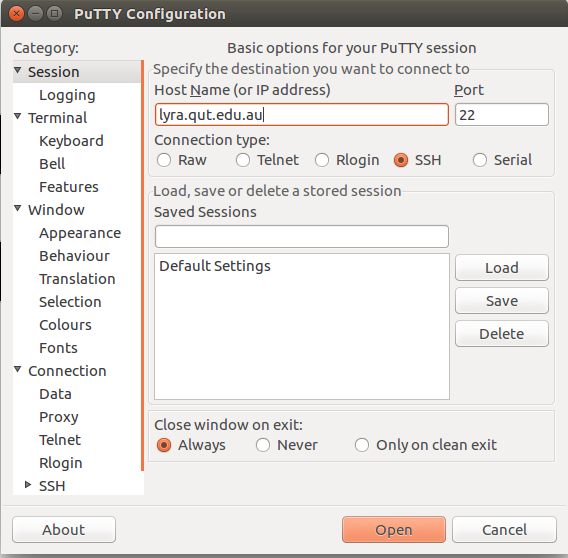
\includegraphics[width=0.5\linewidth]{./figs/putty.png}
  \caption{Example PuTTY window}
  \label{fig:putty}
\end{figure}
%
%
\subsection{Once Logged In}
After following the previous commands you will be logged into the head node of the Lyra HPC cluster. Though you will now be logged in, you have not been allocated any computational resources yet. The head node is available to all users once logged in, and is designed for performing only simple tasks, such as text editing or checking on currently running jobs.
%
%
\par
%
%
\subsection{Transferring Files to HPC}
Now that you have access to HPC, you will want to transfer some code over so you can start running some jobs. There are a few ways to do this, though this guide will cover the easier/most prominent ways to do this.
%
%
\par
%
%
To get your code onto HPC, I would recommend simply using Git and cloning your repo onto HPC. If you are unsure on how to use Git, I would strongly recommend you take some time to learn some basics and start using it for your software projects. Knowledge of Git is not required for this guide, but it will make your software development life significantly better, and allow you to distribute your research much easier.
%
%
\par
%
%
You can clone your repo to HPC via the terminal that is connected to HPC by simply running the command,
\begin{lstlisting}[language=bash, frame=single]
  #change to the home directory
  git clone <remote_url_for_your_repo>
\end{lstlisting}
%
%
It is also helpful to be able to transfer other files to and from HPC. The easiest way to do this is to mount a network directory, so you can copy and paste files to and from HPC just like you would on your desktop/laptop. Instructions on how to do this for Windows, Mac and Linux using SSHFS is provided \href{https://www.digitalocean.com/community/tutorials/how-to-use-sshfs-to-mount-remote-file-systems-over-ssh}{here}. After you install the required programs, you can mount the directory creating a folder on your desktop where you want to mount your HPC files by running the following command,
%
%
\hspace*{-2cm}
\begin{lstlisting}[language=bash, breaklines=true, frame=single]
  #all of this in a single line/command
  sshfs -o allow_other <your_qut_username>@lyra.qut.edu.au:/home/<your_qut_username> <path_to_mount_location_on_desktop>
\end{lstlisting}
% 
%
%

%%% Local Variables:
%%% mode: latex
%%% TeX-master: "main"
%%% End: